\documentclass[landscape]{a0poster}
\usepackage{amsfonts, amsmath, amsthm, amssymb} % For math fonts, symbols and environments
\usepackage{algorithm}
\usepackage[noend]{algpseudocode}
\usepackage{tikz,pgfplots}
\usetikzlibrary{decorations,arrows,shapes,trees,positioning}
\usepackage[position=top,aboveskip=5pt,labelformat=empty]{subfig}
\usepackage{soul}
\usepackage{balance}
\usepackage{xcolor}
\usepackage{listings}

\definecolor{mGreen}{rgb}{0,0.6,0}
\definecolor{mGray}{rgb}{0.5,0.5,0.5}
\definecolor{mPurple}{rgb}{0.58,0,0.82}
\definecolor{backgroundColour}{rgb}{0.95,0.95,0.92}


\protected\def\vvv#1{\leavevmode\bgroup\vbox\bgroup\xvvv#1\relax}

\def\xvvv{\afterassignment\xxvvv\let\tmp= }

\def\xxvvv{%
	\ifx\tmp\@sptoken\egroup\ \vbox\bgroup\let\next\xvvv
	\else\ifx\tmp\relax\egroup\egroup\let\next\relax
	\else
	%\hbox{\tmp}%original
	\hbox to 1.1em{\hfill\tmp\hfill}% centred
	\let\next\xvvv\fi\fi
	\next}


%\pgfplotsset{compat=1.13}

\definecolor{cpu3}{HTML}{F44336}
\definecolor{cpu4}{HTML}{2196F3}
\definecolor{cpu1}{HTML}{4CAF50}
\definecolor{cpu2}{HTML}{FFC107}
\definecolor{gpu3}{HTML}{EF9A9A}
\definecolor{gpu4}{HTML}{90CAF9}
\definecolor{gpu1}{HTML}{A5D6A7}
\definecolor{gpu2}{HTML}{FFE082}

\definecolor{cpu5}{HTML}{9932CC}

\definecolor{sq_b1}{RGB}{37,52,148}
\definecolor{sq_b2}{RGB}{44,127,184}
\definecolor{sq_b3}{RGB}{65,182,196}
\definecolor{sq_b4}{RGB}{127,205,187}
\definecolor{sq_b5}{RGB}{199,233,180}
\definecolor{sq_b5}{RGB}{255,255,204}

\definecolor{sq_r1}{RGB}{189,0,38}
\definecolor{sq_r2}{RGB}{240,59,32}
\definecolor{sq_r3}{RGB}{253,141,60}
\definecolor{sq_r4}{RGB}{254,178,76}
\definecolor{sq_r5}{RGB}{254,217,118}
\definecolor{sq_r6}{RGB}{255,255,178}

\definecolor{sq_g1}{RGB}{0,104,55}
\definecolor{sq_g2}{RGB}{49,163,84}
\definecolor{sq_g3}{RGB}{120,198,121}
\definecolor{sq_g4}{RGB}{173,221,142}
\definecolor{sq_g5}{RGB}{217,240,163}
\definecolor{sq_g6}{RGB}{255,255,204}


\definecolor{div_c1}{RGB}{230,171,2}
\definecolor{div_c2}{RGB}{102,166,30}
\definecolor{div_c3}{RGB}{231,41,138}
\definecolor{div_c4}{RGB}{117,112,179}
\definecolor{div_c5}{RGB}{217,95,2}
\definecolor{div_c6}{RGB}{27,158,119}
\definecolor{div_c7}{RGB}{215,48,39}

%% user command
\newcommand{\mvec}{\textsc{MATVEC}}
\newcommand{\hmvec}{\textsc{HMATVEC}}
\newcommand{\gexchange}{\textsc{GhostExchange}}
\newcommand{\tsort}{\textsc{TreeSort}}
\newcommand{\ssort}{\textsc{SampleSort}}
%\newcommand{\dsort}{\textsc{DistTreeSort}}
\newcommand{\dsort}{\textsc{OptiPart}}
\newcommand{\note}[1]{\noindent\emph{\textcolor{purple}{#1}}}
\algrenewcommand\algorithmicrequire{\textbf{Input:}}
\algrenewcommand\algorithmicensure{\textbf{Output:}}
\algrenewcommand\algorithmicforall{\textbf{parallel for}}
\newcommand{\hilbertcurve}{\textsc{Hilbert }}
\newcommand{\mortoncurve}{\textsc{Morton }}
\newcommand{\octdomain}{\mathcal{N}^3}



\newcommand{\Intel}{Intel\textsuperscript{\textregistered}\xspace}
\newcommand{\snb}{Xeon\texttrademark\xspace}
\newcommand{\xphi}{Xeon Phi\texttrademark\xspace}
\newcommand{\Summit}{\href{https://www.olcf.ornl.gov/summit/}{Summit}}
\newcommand{\Aurora}{\href{http://aurora.alcf.anl.gov/}{Aurora}}
\newcommand{\Stampede}{\href{https://www.tacc.utexas.edu/stampede/}{Stampede}}
\newcommand{\Titan}{\href{https://www.olcf.ornl.gov/titan/}{Titan}}
\newcommand{\Cloudlab}{\href{https://cloudlab.us/}{CloudLab}}

%\theoremstyle{defn}
\newtheorem{defn}{Definition}

\theoremstyle{plain}
\newtheorem{theorem}{Theorem}
\newtheorem{lemma}{Lemma}
\newtheorem{remark}{Remark}

\lstdefinestyle{CStyle}{
    backgroundcolor=\color{backgroundColour},   
    commentstyle=\color{mGreen},
    keywordstyle=\color{magenta},
    numberstyle=\tiny\color{mGray},
    stringstyle=\color{mPurple},
    basicstyle=\footnotesize,
    breakatwhitespace=false,         
    breaklines=true,                 
    captionpos=b,                    
    keepspaces=true,                 
    numbers=left,                    
    numbersep=5pt,                  
    showspaces=false,                
    showstringspaces=false,
    showtabs=false,                  
    tabsize=2,
    language=C
}
\usepackage{geometry}
\geometry{paperwidth=30in,paperheight=40in,margin=2cm}
\pagestyle{empty}
\setcounter{secnumdepth}{0}
% The textpos package is necessary to position textblocks at arbitary 
% places on the page.
\usepackage[]{textpos}
\usepackage{graphicx,wrapfig}
\usepackage{tikz,pgflibraryshapes}
\usetikzlibrary{shapes,arrows,trees,snakes}

\usepackage{amsmath,amssymb}
\usepackage{color}
\usepackage{setspace}
\usepackage{lipsum}
\onehalfspacing


%% SC18 colors
\definecolor{DarkBlue}{rgb}{0.0,0.1255,0.357}
\definecolor{Red}{rgb}{0.655,0.1,0.185}

% see documentation for a0poster class for the size options here
\let\Textsize\normalsize
%\LARGE
%\def\Head#1{\noindent\hbox to \hsize{\hfil\textbf{\LARGE\color{Red}#1}}\medskip}
\def\Head#1{\noindent{\textbf{\LARGE\color{Red} #1}}\medskip}
\def\LHead#1{\noindent{\Large\color{DarkBlue} #1}\bigskip}
\def\Subhead#1{\noindent{\textbf{\Large\color{DarkBlue} #1}}\medskip}
\def\Title#1{\noindent\textbf{{\VeryHuge\color{Red} #1}}}

\def\Subtitle#1{\noindent\textbf{{\Large\color{Red} #1}}}

\parindent=0pt
\parskip=0.5\baselineskip

\TPGrid[0in,0in]{30}{40}    %(horizontal unit 1in, vertical unit 1in)
\newcommand{\argmax}[1]{\ensuremath{\arg \,\underset{#1}{\max}\;}}


%%%%%%%%% parameters to set column width and other spacing
\def \tpcoulmnwidth{9} 
\def \tpcolIX{11.5}
\def \tpcoulmgap{1.0}
\def \tpblockX{0.5}



\begin{document}

% \tikz[remember picture,overlay] \node[opacity=0.3, inner sep=0pt] at (current page.center){\includegraphics[width=\paperwidth,height=\paperheight]{r1_img5}};

\begin{textblock}{20}(-1,-1) 
\resizebox{18\TPHorizModule}{!}{\includegraphics{../sc18/figs/TopLeft}}
\end{textblock} 

\begin{textblock}{20}(11,38.4) 
	\resizebox{18\TPHorizModule}{!}{\includegraphics{../sc18/figs/BottomRight}}
\end{textblock} 

\begin{textblock}{2}(21,3.6) %<<<
\resizebox{2.5\TPHorizModule}{!}{\includegraphics{../sc18/figs/Ulogo_cmyk}}
\end{textblock} %>>>




%% {{{ Headings 

%\begin{textblock}{5}(14.8,-0.6) %<<<
%	\resizebox{5\TPHorizModule}{!}{\includegraphics{../sc18/figs/dendro}}
%\end{textblock} %>>>



\begin{textblock}{25}(0,1.2) %<<<
	\Title{Common Subexpression Elimination with Subtree Isomporphisms }
\end{textblock} %>>>


\begin{textblock}{20}(2.0,4) %<<<
\LHead{{\huge Robert King}, {\Huge Mentors: Hari Sundar, Milinda Fernando}
\hfil\\[1ex]
\textsl{University of Utah}}
\end{textblock}



%% }}}

% COLUMN 1 {{{
	\begin{textblock}{14}(0,6)
	{\color{DarkBlue}\hrule}\medskip	
	\Subhead{Motivation} %%===================================
	
	\vspace{-0.2in}
	The purpose of this work is to improve the run time of the simulation of black hole collisions as seen in the Dendro-Gr framework. The BSSN equations and several other simulation codes consist of several complex partial differential equations and to model these equations the value of each variable is computed once per a time step in the model. The project presented aims to provide a method to increase cache utilization to increase runtime performance.
	\end{textblock} 	

	\begin{textblock}{14}(0, 10.5)
		{\color{DarkBlue}\hrule}\medskip
		\Subhead{Contributions}
		\vspace{-0.2in}
		\begin{itemize}
			\item \textbf{Wavelet Adaptive GR}. 
			This is the first highly adaptive computational fully relativistic---i.e., including the full Einstein equations---code with 
			an \textcolor{blue}{arbitrary localized unstructured} wavelet based adaptive mesh.
			\item \textbf{Automatic code-generation}. Given the complexity of the Einstein equations, we have developed an automatic code generation framework for GR using \texttt{SymPy} that automatically generates architecture-optimized codes which helps to improve code portability. 
			\item \textbf{Performance}. We developed a new parallel search algorithm, \tsearch~ to improve the efficiency of octree meshing. We also developed efficient \texttt{unzip} and \texttt{zip} operations to allow the application of the core computational kernels on small process-local regular blocks which leads to greater performance and code portability (i.e. GPU architectures).
			\item \textbf{Visualization}. 
			Code is able to represent expression trees with Graphiz and visualize expression tree staging			
			\item \textbf{Implementation} \dendro~ is implemented in \textsc{Python} using \texttt{SymPy} for the autocode generation for the partial differntial equations. The Code is freely available at \\ \texttt{\small https://github.com/paralab/Dendro-GR} under the MIT license.
		\end{itemize}
	\end{textblock} 
% }}}

\begin{textblock}{30}(0,21.5)
	{\color{DarkBlue}\hrule}\medskip
	\Head{Method} %%===================================

	\begin{textblock}{14}(0,0.2)
% \begin{itemize}
% 	\item For accurate simulations, the spatial discretization $dx\leq min(m_1,m_2)/10$ where $m_1, m_2$ are the masses of the black holes.  
% 	\item \textbf{Mass ratio Vs. Number of grid points} : $N \propto q^3$ where $q=m_1/m_2$. 
% 	\item \textbf{Feasibility} For IMRIs to be feasible we need highly localized adaptive grids. (compared to structured adaptivity) 
% \end{itemize}
% A key reason to develop scalable codes is that
% as the relative differences in masses becomes larger ($\sim 100\times$), the computational
% requirements will grow significantly, potentially requiring exascale resources.
%A simple calculation illustrates how spatial resolution requirements increase
%with the mass ratio, $q$. 
%A convenient measure for the size of a black hole is the radius of its event horizon, which is proportional to its mass.

%In a black hole binary, the mass of the smallest black hole effectively sets the minimum length scale for the simulation. The total mass of the binary
%$M = m_1 + m_2$ is a global scaling parameter and is typically fixed to  a constant value. 
%Then the mass of the smaller black hole can be written $m_2 = M/(q+1)$, showing that the minimum resolution scale for the
%binary is inversely proportional to the mass ratio. In $3d$ the number of points required to resolve the smallest black hole
%grows as $q^3$.

% This presents both a challenging problem in computational relativity
% as well as a challenge for high-performance computing.
% The successful scaling of our code is a first step in this direction.
\end{textblock}
%\vspace{-0.5in}



\begin{textblock}{14}(14.5,-0.5)
	\Subhead{Rebuilding}% (ORNL's \Titan~ upto $131K$ cores)} 

	\vspace{-0.25in}
	The rebuilding phase takes the results from the staging process and rebuilds the expression tree. In order of importance the rebuilding phase must preserve the correct final answers, maximize cache effectiveness, and minimize the total number of temporary variables used. The current strategy is to use a dynamic programming approach. Dynamic programming will also allow for the rebuilding process to scale effectively. Once complete, these results will be measured experimentally. Once a proof of concept has been completed the rebuilding process will take in parameters such as memory architecture, and L1 cache size to optimize the calculations for each machine. Once the rebuilding process is completed a parser will be created to transform the original SymPy autogenerated code to reflect the updated expression tree.
	\begin{textblock}{12}(2,1)
	%\begin{figure}
	%	\centering
	%	\resizebox{12\TPHorizModule}{!}{{\includegraphics{../sc18/plots/weak_r10}}}
	%	\vspace{-0.2in}
	%\end{figure}	
	\end{textblock}	
\end{textblock}
	

\begin{textblock}{8}(8.5,4)

%\begin{figure}
%		\centering
%		\resizebox{!}{7\TPHorizModule}{\includegraphics{../sc18/plots/strong_r10}}
%\end{figure}	
\end{textblock}


%\begin{textblock}{8}(0,9.2)
%\Subhead{Strong scaling results $\rightarrow$}

%\vspace{-0.3in}
%Strong scaling results in ORNL's \Titan~for a single RK step (averaged over 10 steps) 
%with derivative computation (\texttt{deriv}), right hand side( {\texttt rhs}) computation, \texttt{unzip} cost and communication cost (\texttt{comm}) 
%for a fixed problem size of $10.5B$ unknowns where the number of cores ranging from $4,096$ to $65,536$ cores on $4096$ nodes. %Note that for strong scaling %results re-meshing is disabled in order to keep the problem size fixed.
%\end{textblock}


\begin{textblock}{29}(-0.25,8.5)
	\begin{figure}
%		\centering
%		\begin{subfigure}{0.33\textwidth}
%			\includegraphics[width=0.9\textwidth]{../sc18/figs/img_slice_chi_r1.png}
%			\caption{$q=1$}
%		\end{subfigure}
%		\begin{subfigure}{0.33\textwidth}
%			\includegraphics[width=0.9\textwidth]{../sc18/figs/img_slice_chi_r10.png}
%			\caption{$q=10$}
%		\end{subfigure}
%		\begin{subfigure}{0.33\textwidth}
%			\includegraphics[width=0.9\textwidth]{../sc18/figs/img_slice_chi_r100.png}
%			\caption{$q=100$}
%		\end{subfigure} \hfil
		\begin{subfigure}{0.33\textwidth}
			\includegraphics[width=\textwidth]{../sc18/figs/img_slice_level_r1.png}
			\caption{\large $q=1$}
		\end{subfigure}
		\begin{subfigure}{0.33\textwidth}
			\includegraphics[width=\textwidth]{../sc18/figs/img_slice_level_r10.png}
			\caption{\large $q=10$}
		\end{subfigure}
		\begin{subfigure}{0.33\textwidth}
			\includegraphics[width=\textwidth]{../sc18/figs/img_slice_level_r100.png}
			\caption{\large $q=100$}
		\end{subfigure}
	%	\caption{\small Time step snapshots of the binary black hole problem of black hole mass ratios $1, 10 \& 100$ where we in the top row we plot the \BSSN~variable $\chi$ in the lower row we plot the WAMR grids for each case at that specific instance. \label{fig:large_q}}
	\end{figure}
\end{textblock}


\begin{textblock}{14}(0,3)
	\Subhead{Staging}% (ORNL's \Titan~ upto $131K$ cores)} 

	\vspace{-0.25in}
	Staging is focused on finding variable reuse within the partial differential equations. The first problem is to create an expression tree from the partial differential equations generated from the SymPy auto generated code. 
	Once the expression tree is created, subtree isomorphism analysis can begin. This will be a bottom up approach that considers the values used in each leaf node in addition to finding similar tree structure. Each node within the tree will keep track of all the leaf values that it depends on. Set similarity will be used as a precondition before calculating the more expensive tree isomorphism. By the end of the Staging Process the most common subexpressions will be identified. Each expression will be valued depending on the number of leaf node dependents, to mitigate the total number of temporary variables, and the number of times each expression appears, to maximize data reuse.

	
\end{textblock}

\end{textblock}
%%=== === === SYMBOLIC

\begin{textblock}{14}(14.5,6)
	{\color{DarkBlue}\hrule}\medskip
	\Subhead{Symbolic code generation for \BSSN~ equations}
	\begin{figure}
%	 \noindent\fbox{
			\begin{minipage}[t]{.48\textwidth}
				\small
				\begin{eqnarray*}
					\partial_t \alpha &=&  \mathcal{L}_\beta\alpha - 2 \alpha K, \\
					\partial_t \beta^i &=& \lambda_2 \beta^j\,\partial_j\beta^i + \frac{3}{4} f(\alpha) B^i\\
					\partial_t B^i  &=& \partial_t \tilde\Gamma^i  - \eta B^{i}   + \lambda_3 \beta^j\,\partial_j B^i - \lambda_4 \beta^j\,\partial_j \tilde\Gamma^i \\
					\partial_t \tilde \gamma_{ij} &=&  \mathcal{L}_\beta\tilde{\gamma}_{ij} -2 \alpha \tilde A_{ij}, \\
					\partial_t \chi &=& \mathcal{L}_\beta\chi + \frac{2}{3}\chi \left(\alpha K -  
					\partial_a \beta^a\right)\\
					\partial_t \tilde A_{ij} &=& \mathcal{L}_\beta\tilde{A}_{ij} + \chi \left(-D_i D_j \alpha +
					\alpha R_{ij}\right)^{TF} +\nonumber \\
					&\,&\alpha \left(K \tilde A_{ij} -
					2 \tilde A_{ik} \tilde A^{k}_{\,j}\right), \label{eq:at_evol}\\
					\partial_t K &=& \beta^k\partial_kK- D^i D_i \alpha + \\
					&\,&\alpha \left(\tilde A_{ij}\tilde
					A^{ij} +\frac{1}{3}K^2\right),\\
					\partial_t \tilde \Gamma^i &=& \tilde \gamma^{jk} \partial_j
					\partial_k \beta^i + \frac{1}{3} \tilde \gamma^{ij} \partial_j
					\partial_k \beta^k + \beta^j \partial_j \tilde \Gamma^i - \nonumber \\
					&\,&\tilde
					\Gamma^j \partial_j \beta^i + 
					\frac{2}{3}\tilde \Gamma^i \partial_j
					\beta^j - 2 \tilde A^{i j}\partial_j \alpha + \nonumber \\
					&\,& 2 \alpha \left(\tilde
					{\Gamma^i}_{jk} \tilde A^{jk} - \frac{2}{3 \chi} \tilde A^{ij}\partial_j \chi -
					\frac{2}{3} \tilde \gamma^{ij} \partial_j K\right) \\
					% ~ &~ & ~\\
				\end{eqnarray*}
			\end{minipage}% This must go next to `\end{minipage}`
%		}
	\begin{minipage}[t]{.5\textwidth}
\small
%frame=single,framesep=1pt,
\begin{minted}[frame=single,framesep=1pt,bgcolor=yellow!10]{python}
	
   from DENDRO_sym import *
   a_rhs = Dendro.Lie(b, a) - 2*a*K
   b_rhs = [3/4 * f(a) * B[i] + 
   l2*vec_j_del_j(b, b[i]) for i in e_i]
   l2*vec_j_del_j(b, b[i]) 
   for i in e_i]
   B_rhs = [Gt_rhs[i] - eta * B[i] + 
   l3 * vec_j_del_j(b, B[i]) - 
   l4 * vec_j_del_j(b, Gt[i]) 
   for i in e_i]
   gt_rhs =  Dendro.Lie(b, gt) - 2*a*At
   chi_rhs = Dendro.Lie(b, chi) + 
   2/3*chi*(a*K - del_j(b)) 
   At_rhs = Dendro.Lie(b, At) + chi *
   Dendro.TF(-DiDj(a) + 
   a*Dendro.Ricci) +
   a*(K*At -2*At_ikAtKj)
   K_rhs = vec_k_del_k(K) - DIDi(a) +
   a*(1/3*K*K + A_ij_A_IJ(At)) 
   
\end{minted}
\end{minipage}
%\caption{\label{fig:symb} \small The left panel shows the \BSSN ~formulation of the Einstein equations. These are tensor equations, with indices $i,j,\ldots$ taking the values $1, 2, 3$. On the right we show the \texttt{{\dendro\_sym}} code for these equations. \texttt{\dendro\_sym} uses \texttt{SymPy} and other tools to generate optimized C++ code to evaluate the equations. Note that $\mathcal{L}_\beta,\ D,\ \partial$ denote Lie derivative, covariant derivative and partial derivative respectively, and we have excluded $\partial_t\Gamma^i$ from \texttt{\dendro\_sym} to save space.}
%\label{fig:bssneqs}
\vspace{-0.15in}
\end{figure}
The left panel shows the \BSSN ~formulation of the Einstein equations. These are tensor equations, with indices $i,j,\ldots$ taking the values $1, 2, 3$. On the right we show the \texttt{{\dendro\_sym}} code for these equations. \texttt{\dendro\_sym} uses \texttt{SymPy} and other tools to generate optimized C++ code to evaluate the equations. Note that $\mathcal{L}_\beta,\ D,\ \partial$ denote Lie derivative, covariant derivative and partial derivative respectively, and we have excluded $\partial_t\Gamma^i$ from \texttt{\dendro\_sym} to save space.

For additional details please refer to {\bf Massively Parallel Simulations of Binary Black Hole Intermediate-Mass-Ratio Inspirals}, Milinda Fernando, David Neilsen, Hyun Lim, Eric Hirschmann, Hari Sundar, \url{https://arxiv.org/abs/1807.06128}.
\end{textblock}





% %% === === === NLSM
% \begin{textblock}{14}(14.5,5)
% 	{\color{DarkBlue}\hrule}\medskip
% 	\Subhead{Simple example: Non-linear sigma model}
	
% 		\begin{figure}
% %		\noindent\fbox{
% 			\begin{minipage}[t]{.48\textwidth}
% %				\small
% 				\begin{eqnarray*}
% 				\partial_t\phi &=& \Delta \chi -\frac{\sin(2\chi)}{{\norm{x}_2}^2} \\
% 				\partial_t\chi &=& \phi 
% 				\end{eqnarray*}
% 			\end{minipage}% This must go next to `\end{minipage}`
% %		}
% 		\begin{minipage}[t]{.5\textwidth}
% 			\small
% %frame=single,framesep=2pt,
% \begin{minted}[frame=single,framesep=1pt,bgcolor=yellow!10]{python}
%  from DENDRO_sym import *
%  phi_rhs = sum(d2(i,i,chi)for i in dendro.e_i) 
%  		- sin(2*chi)/r**2
%  chi_rhs = phi
% \end{minted}
% 		\end{minipage}
% 		%\caption{\label{fig:symb} \small The left panel shows the \BSSN ~formulation of the Einstein equations. These are tensor equations, with indices $i,j,\ldots$ taking the values $1, 2, 3$. On the right we show the \texttt{{\dendro\_sym}} code for these equations. \texttt{\dendro\_sym} uses \texttt{SymPy} and other tools to generate optimized C++ code to evaluate the equations. Note that $\mathcal{L}_\beta,\ D,\ \partial$ denote Lie derivative, covariant derivative and partial derivative respectively, and we have excluded $\partial_t\Gamma^i$ from \texttt{\dendro\_sym} to save space.}
% 		%\label{fig:bssneqs}
% 		\vspace{-0.15in}
% 	\end{figure}
% 	\vspace{0.7in}
	
% 	\begin{figure}
% 		\begin{subfigure}{0.33\textwidth}
% 			\includegraphics[width=0.9\textwidth]{../sc18/figs/nlsmB0.png}
% 			\caption{step=0}			
% 		\end{subfigure}
% 		\begin{subfigure}{0.33\textwidth}
% 			\includegraphics[width=0.9\textwidth]{../sc18/figs/nlsmB7.png}
% 			\caption{step=7}			
% 		\end{subfigure}
% 		\begin{subfigure}{0.33\textwidth}
% 			\includegraphics[width=0.9\textwidth]{../sc18/figs/nlsmB11.png}
% 			\caption{step=11}
% 		\end{subfigure}\hfil
% 		\begin{subfigure}{0.33\textwidth}
% 			\includegraphics[width=0.9\textwidth]{../sc18/figs/nlsmB16.png}
% 			\caption{step=16}			
% 		\end{subfigure}
% 		\begin{subfigure}{0.33\textwidth}
% 			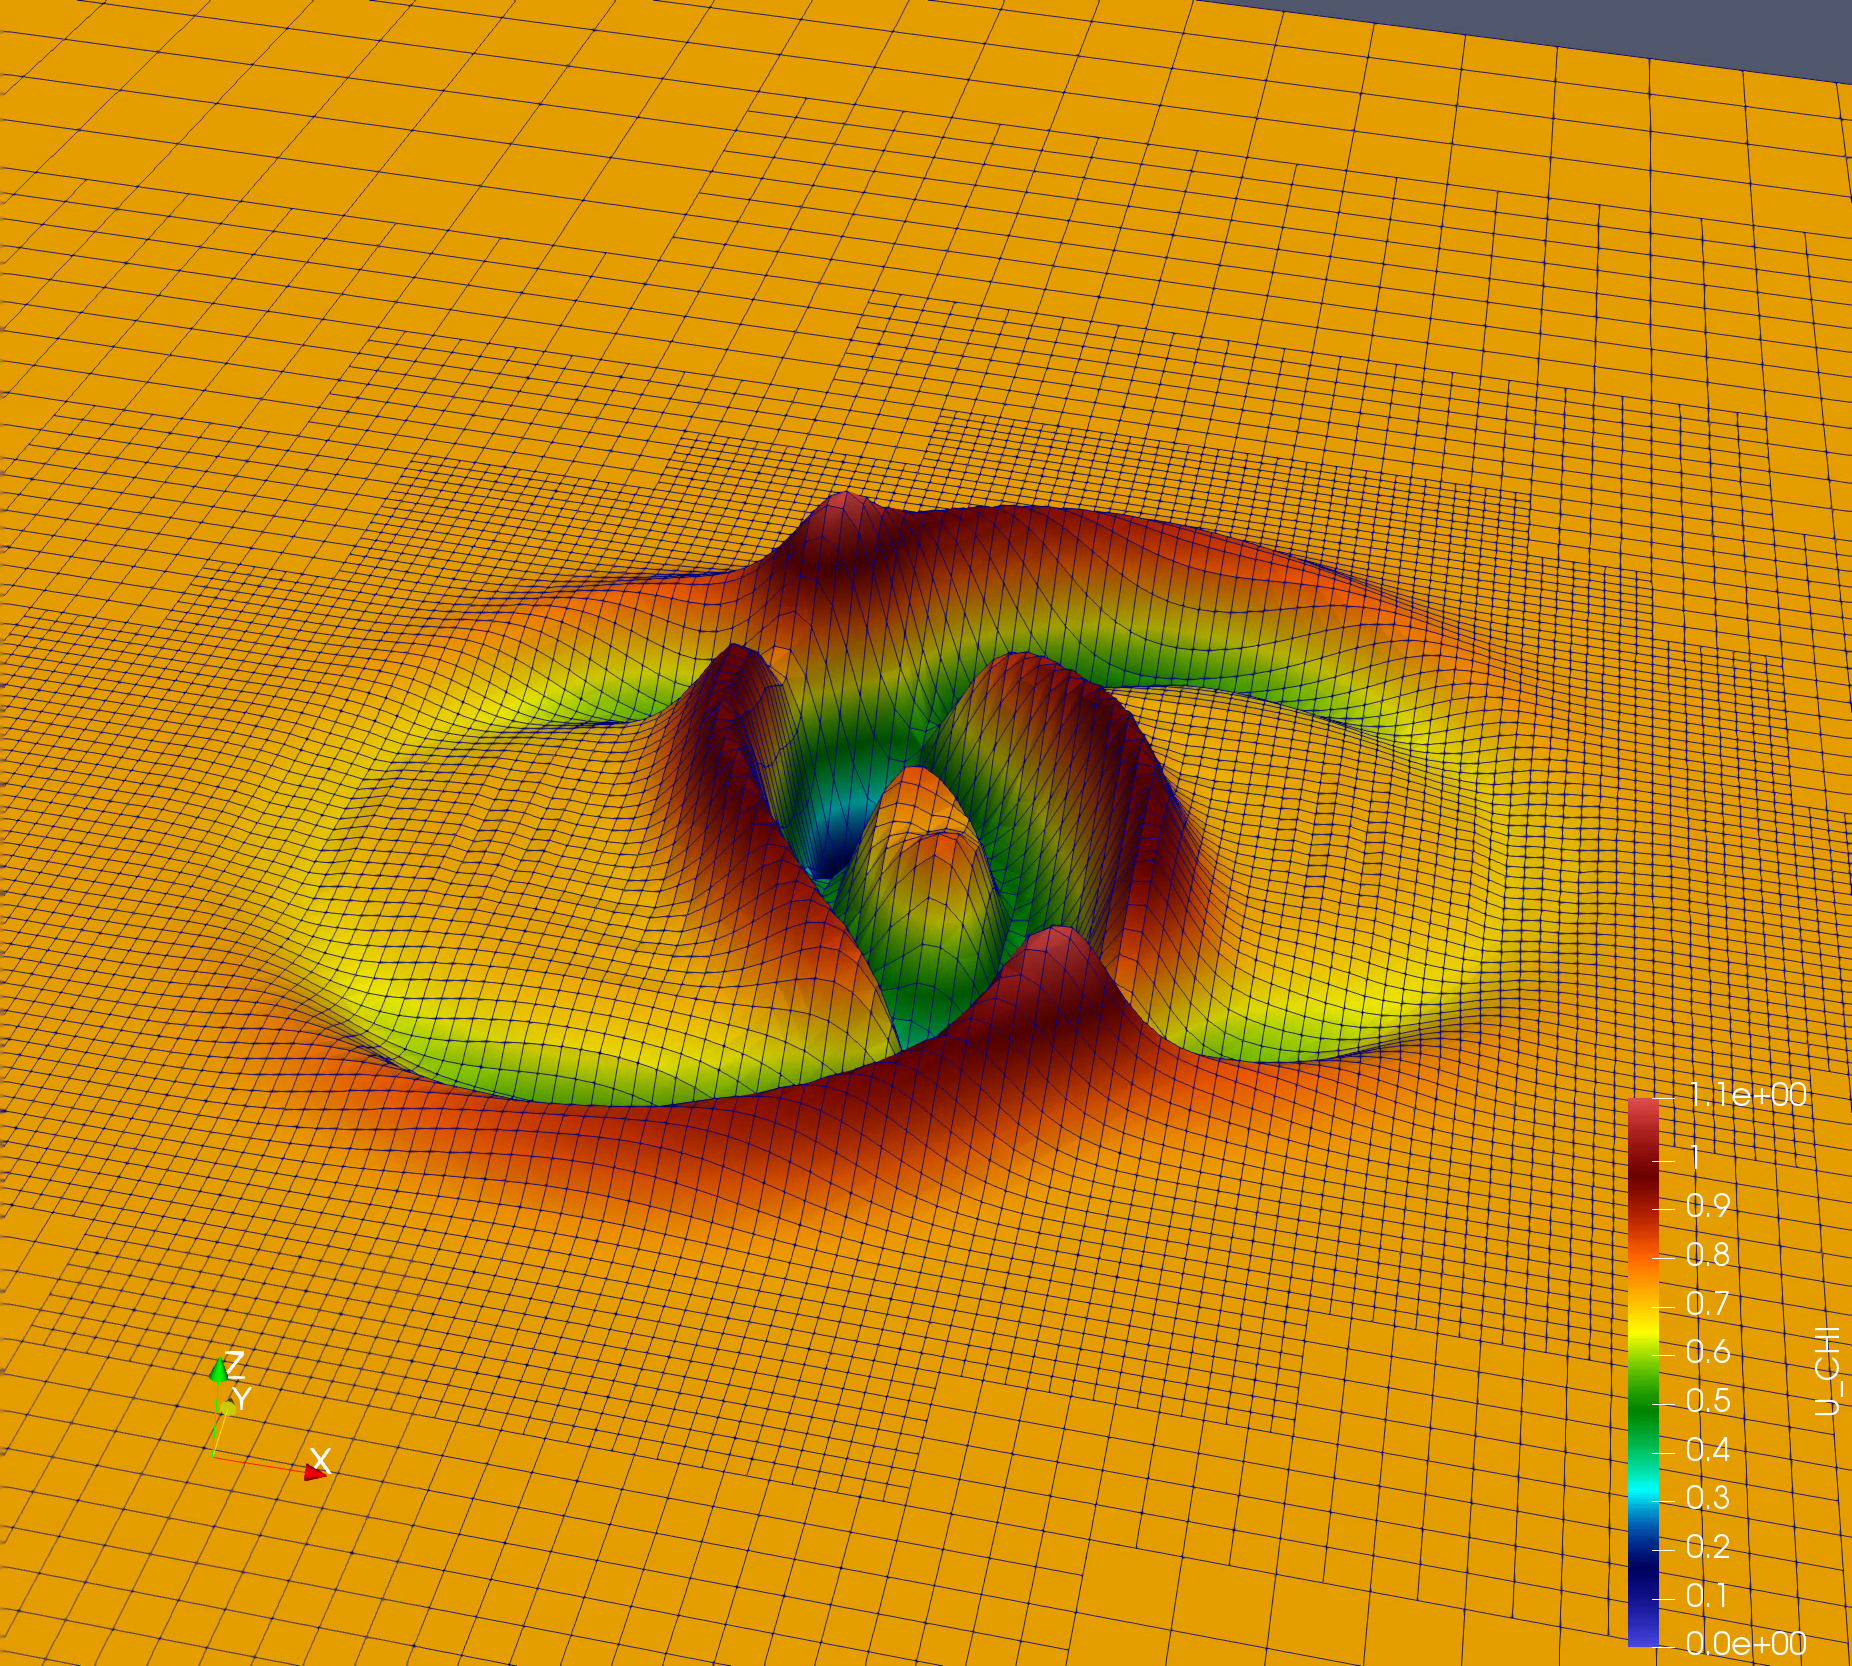
\includegraphics[width=0.9\textwidth]{../sc18/figs/nlsmB23.png}
% 			\caption{step=23}
% 		\end{subfigure}
% 		\begin{subfigure}{0.33\textwidth}
% 			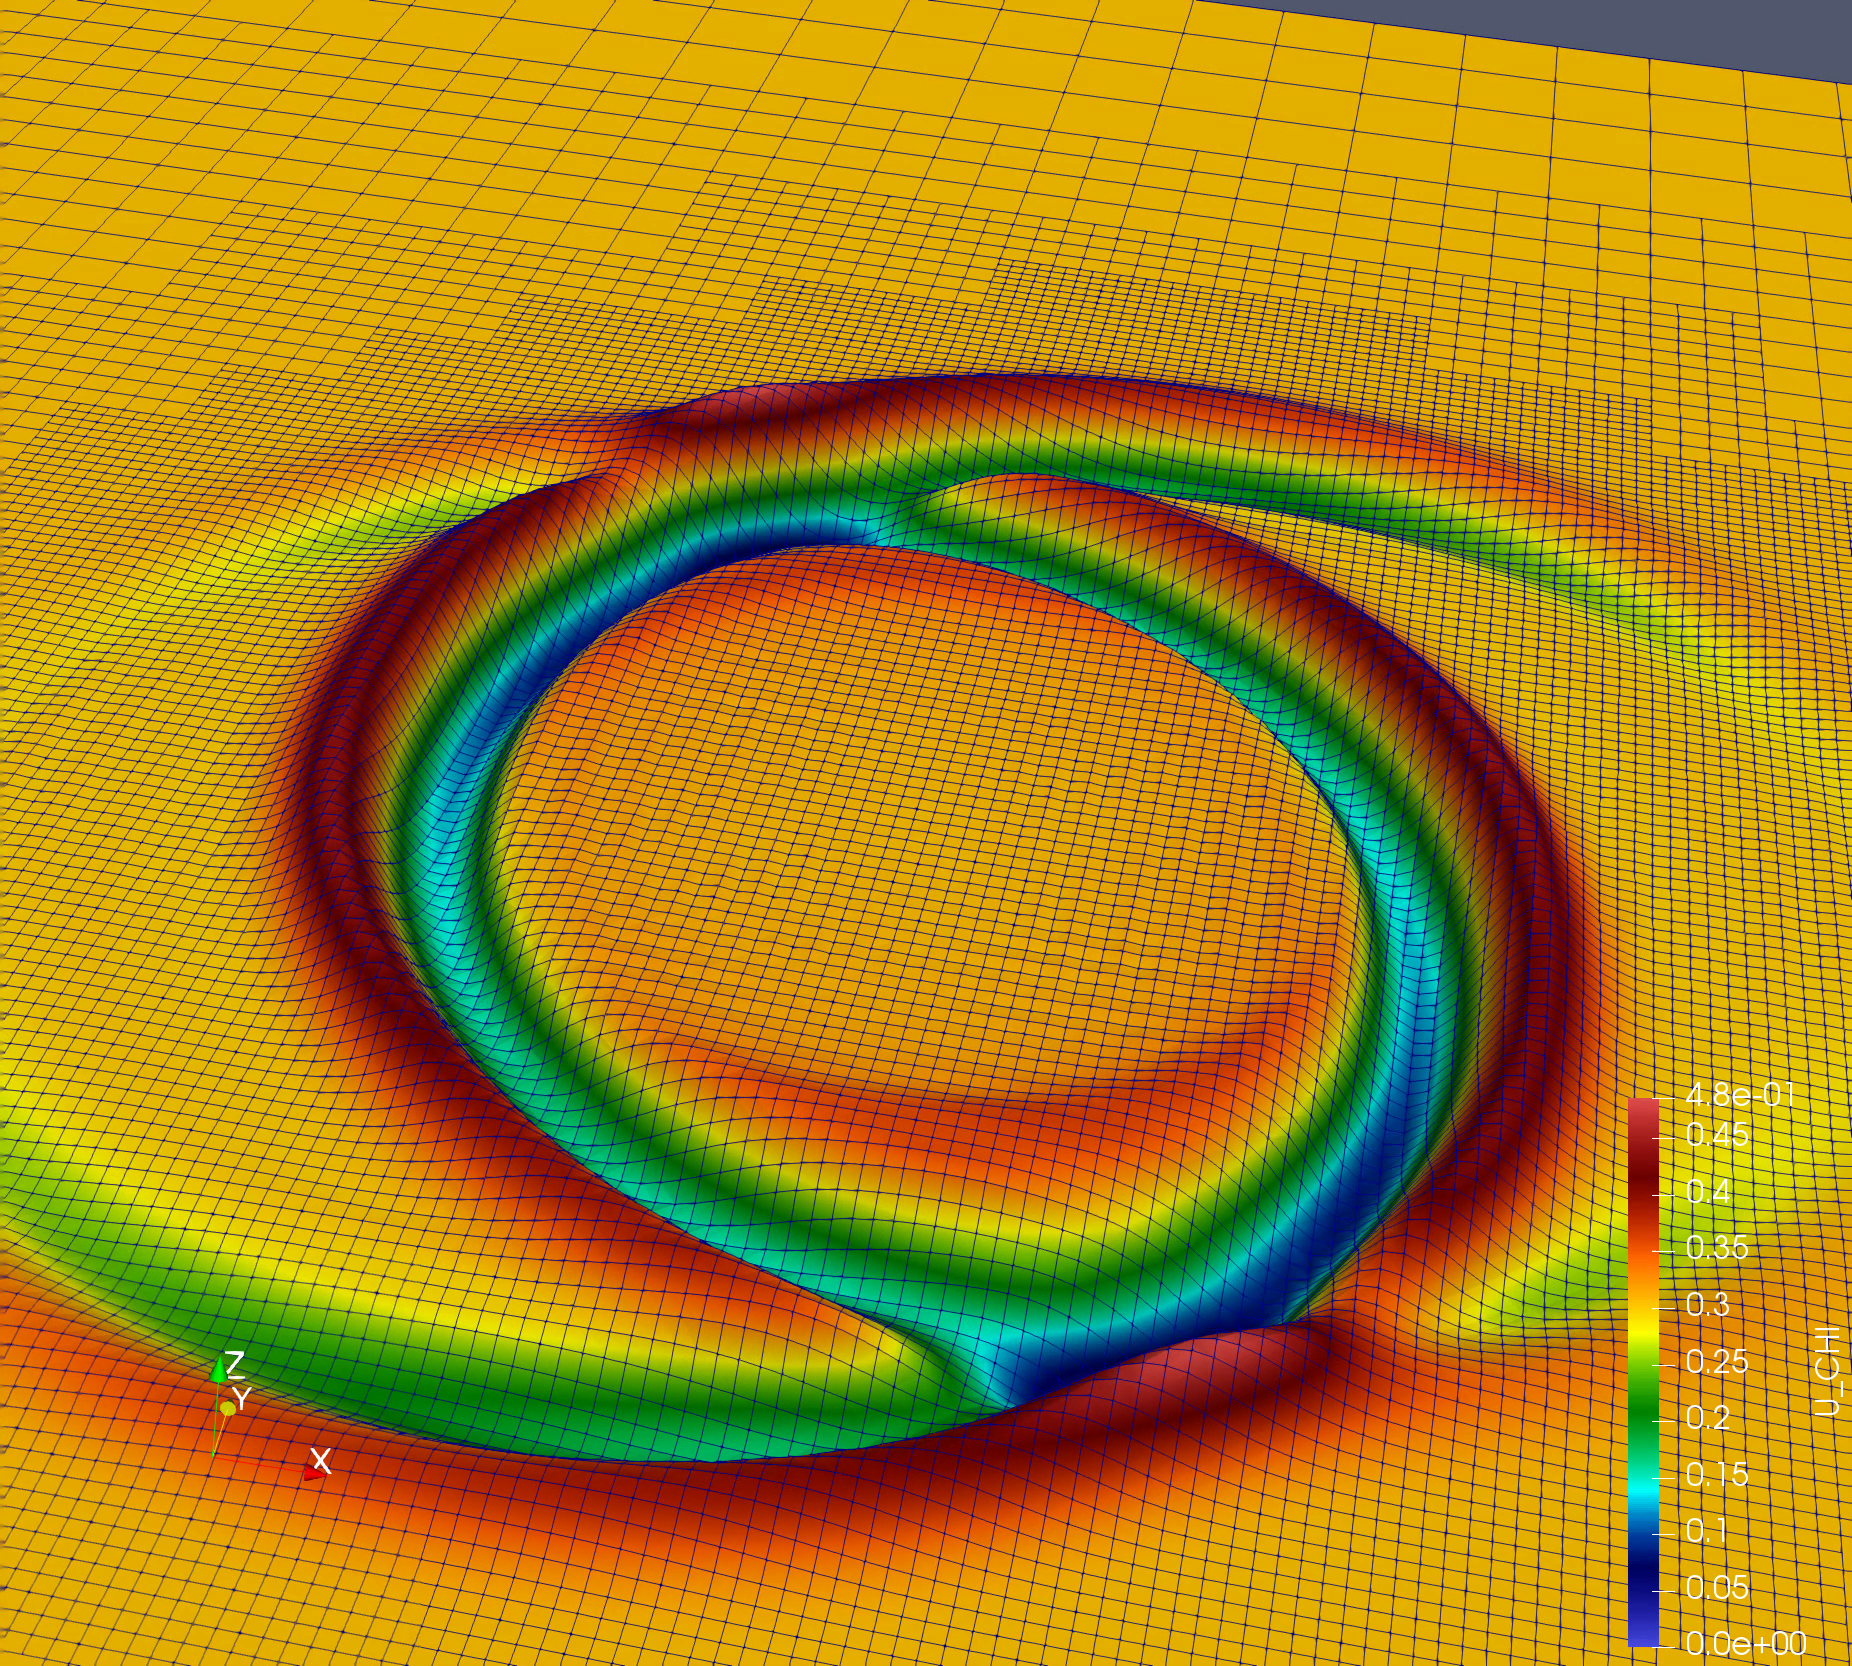
\includegraphics[width=0.9\textwidth]{../sc18/figs/nlsmB44.png}
% 			\caption{step=44}
% 		\end{subfigure}
% 		\caption{Time step snapshots of a $z$ plane slice of $3D$ \NLSM~ with two initial Gaussian distributions with Runge-Kutta time stepping scheme. Note that how the mesh refines (based on the WAMR) as the waves 
% 			propagate away from the origin.   \label{fig:nlsmB}}
% 		\vspace{-0.2in}
% 	\end{figure}
	
% \end{textblock}



% % COLUMN 2 {{{
% 	\begin{textblock}{14}(14.5,5)
% 	{\color{DarkBlue}\hrule}\medskip
% 	\Head{Motivation}
% 	\end{textblock} 
% % }}}


%% =========================

\end{document}

